\section{Descrizione del progetto}
Il progetto scritto in Scala prevede di andare ad affiancare, alla macchinetta del caffè gestita in ASMETA, un distributore automatico di bevande energetiche.

In particolar modo si è progettato un sistema con queste specifiche:
\begin{itemize}
	\item Ogni distributore automatico può essere impostato, in fase di installazione, per funzionare in una lingua piuttosto che in un'altra: nel codice è gestitata solamente la possibilità di introdurre distirbutori automatici in \textbf{lingua italiana} e in \textbf{lingua inglese}.
	\item Ogni ditributore è riconosciuto tramite un identificativo univoco (\textbf{ID}).
	\item Questa tipologia di distributori sono in grado di erogare le seguenti bevande energetiche (\textit{energy drink}):
	\begin{itemize}
		\item \textbf{RedBull};
		\item \textbf{Monster};
		\item \textbf{Gatorade};
		\item \textbf{Italian} (particolare energy drink \textit{made in Italy}).
	\end{itemize}
	Ognuno di questi prodotti sarà caratterizzato dai seguenti campi descrittivi:
	\begin{itemize}
		\item \textbf{Prezzo};
		\item \textbf{Volume} (espresso in cl);
		\item\textbf{Data di scadenza};
		\item Insieme di \textbf{tags}, che permettono di esprimere le caratteristiche e gliusi principali di ogni tipologia di energy drink (ovviamente, ogni lattina di RedBull, per esempio, avrà lo stesso insieme di tags).
		\item \textbf{Valore nutrizionale} indicato teramite tre possibili step
		\begin{itemize}
			\item \textbf{Ipercalorico}
			\item \textbf{Normocalorico}
			\item \textbf{Ipocalorico}
		\end{itemize}
	\end{itemize}
\end{itemize}

Ogni distributore andrà ad offrire le seguenti funzionalità:
\begin{itemize}
	\item \textbf{Acquisto dei prodotti} disponibili, \textbf{regalando i prodotti scaduti}: in particolare la macchinetta sarà in grado di fornire resto esatto al cliente (oppure tutta la somma di denaro inserita nel caso di prodotto scaduto).
	\item \textbf{Stampa dell'elenco dei prodotti disponibili} all'interno del distirbutore, unitamente al \textbf{numero di pezzi disponibili}, come si vede in figura ~\ref{fig:AvailableProducts}.
	\begin{figure}[h]
		\centering
		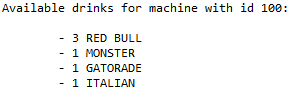
\includegraphics[width=0.4\textwidth]{Immagini/ShowVendingMachine.png}
		\caption{Prodotti disponibili}
		\label{fig:AvailableProducts}
	\end{figure}
	\item Possibilità di \textbf{cercare un prodotto tramite tag}, per poter così trovare l'energy drink più adatto ad ogni specifica evenienza
	\item \textbf{Aggiunta di lattine} di energy drink all'interno del distributore: 
	
	
	TODO: move in another section nello specifico, l'aggiunta di un nuovo prodotto, avviene all'interno di una struttura definita come un array di Queue (ovvero una matrice), che non fa altro che andare a riprodurre la fisionomia di un distirbutore reale.
\end{itemize}

\section{Costrutti utilizzati}
\begin{itemize}
	\item Traits (sezione ~\ref{sec:traits});
	\item Comando \textit{filter} (sezione ~\ref{sec:filter})
	\item Match e Sealed (sezione ~\ref{sec:match_sealed})
\end{itemize}

\newpage
\section{Gerarchia delle classi e trait}
\label{sec:traits}
Nella applicazione realizzata sono stati realizzata due gerarchie facendo uso dei \textit{\textbf{trait}}: i trait in Scala corrispondono alle interfaccie in Java, ovvero permettono di definire la firma di ogni classe che ne implementa la struttura.

Nel nostro caso abbiamo due strutture gerarchiche, gestite tramite traits, mostrate con un grafo ad "albero" nell'immagine seguente (figura ~\ref{fig:classi&traits}).

\begin{figure}[h]
	\centering
	\subfloat[][\emph{Energy drink}]
	{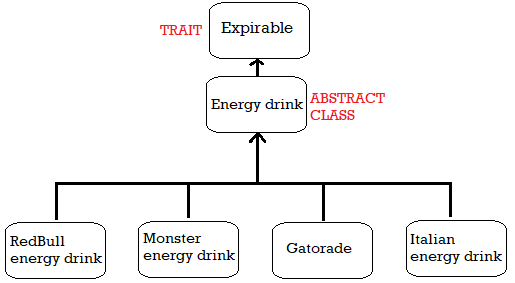
\includegraphics[width=.45\textwidth]{Immagini/EnergyDrink.png}} \quad
	\subfloat[][\emph{Expirable trait}]
	{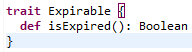
\includegraphics[width=.35\textwidth]{Immagini/ExpirableTrait.png}} \\
	\subfloat[][\emph{Vending machine}]
	{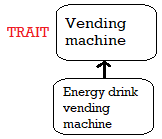
\includegraphics[width=.25\textwidth]{Immagini/VendingMachine.png}} \quad
	\subfloat[][\emph{Vending machine trait}]
	{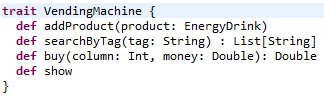
\includegraphics[width=.45\textwidth]{Immagini/VendingMachineTrait.png}}
	\caption{Classi e trait}
	\label{fig:classi&traits}
\end{figure}

Il primo albero gerarchico rappresenta la struttura che "governa" l'insieme dei possibili energy drink: ogni energy drink astratto eredita da \textit{Expirable} la possibilità di "scadere", che, grazie all'\textit{override} implementa direttamente nell'interfaccia astratta, dato che è uguale per ogni tipologia di energy drink concreta.

Il secondo albero gerarchico invece rappresenta l'appartenenza dell'unica tipologia di distributori trattati in questa applicazione (quelli di energy drink), ad un'interfaccia comune a tutte le possibili tipologie di distributori.

\newpage
\section{Filter}
\label{sec:filter}
Per quanto riguarda la funzionalità di ricerca delle bevande in base ai tag, è stata utile l'istruzione \textit{object oriented} \textit{filter}: in questo modo l'utente, in base alle diverse necessità (per esempio: studio intenso), può cercare l'energy drink più adatto.

Il comando di filter è utile nel momento in cui si vogliono filtrare gli elementi di una certa collezione (lista, array, vettore etc), andando a crearne una nuova contenente solamente gli elementi che rispettano il criterio di filtraggio definito in maniera custom (questo criterio è passato sotto forma di \textit{closures}, ovvero una funzione definita localmente "\textit{al volo}").

Nella nostra applicazione siamo andati a filtrare l'elenco dei tag di ogni prodotto: il filtraggio è stato pensato per mantenere solamente i tag contenenti al loro interno il tag cercato dall'utente tramite tastierino di input.

\begin{figure}[h]
	\centering
	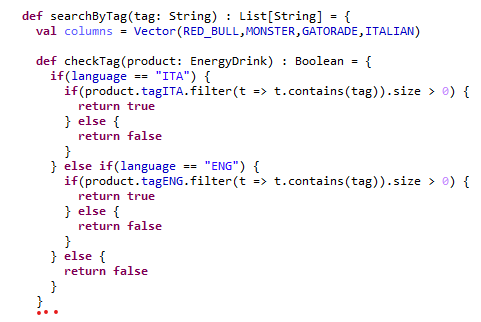
\includegraphics[width=0.55\textwidth]{Immagini/Filter.png}
	\caption{Utilizzo comando \textit{filter}}
	\label{fig:filter}
\end{figure}

\begin{figure}[h]
	\centering
	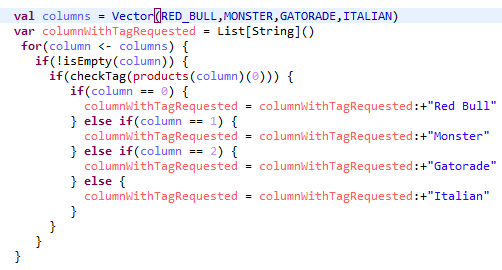
\includegraphics[width=0.55\textwidth]{Immagini/RicercaTag.png}
	\caption{Ricerca del tag su ogni possibile prodotto con \textit{checkTag}}
	\label{fig:filterSearch}
\end{figure}

Come si vede in figura ~\ref{fig:filter}, in base alla tipologia di lingua con cui il distributore è stato impostato, si va a cercare, \textbf{per ogni prodotto disponibile} (figura ~\ref{fig:filterSearch}), nei rispettivi tag, solamente quelli che contengono la parola chiave cercata dall'utente.

In particolare, se il risultato dell'operazione di filter è un vettore con una lunghezza maggiore di 0, significa che il prodotto in esame soddisfa il tag cercato, e quindi può essere mostrato all'utente. 

Questa operazione di filtraggio viene poi ripetuta per ogni tipologia di prodotto disponibile, ovvero per ogni colonna (dato che ogni prodotto ha lo stesso set di tags).

Una volta effettuato il filtraggio \textbf{ho considerato solamente i prodotti il cui risultato dall'operazione di filter non fosse un vettore vuoto}: questo corrisponde infatti al prendere solamente i prodotti che contengono il tag cercato, notificando poi all'utente la loro tipologia, tramite una stampa a display.

\section{Match - sealed}
\label{sec:match_sealed}
\subsection{Match}
Il \textit{pattern match} rappresenta una struttura per verificare il valore assunto da una variabile, tramite un pattern: si tratta in sostanza di una versione leggermente più potente del construtto \textit{switch} di Java.

Nell'applicazione si è pensato di andare ad utilizzare il \textit{pattern matching} in due situazioni:
\begin{itemize}
	\item \textit{Pattern guard}: nell'andare a definire se un prodotto è considerabile come normo, ipo o iper calorico, si è fatto uso di un pattern guard, sfruttando anche la potenzialità aggiuntiva di poter aggiungere una condizione dopo il pattern, tramite la dicitura \textit{if<boolean expression>}, che permette di rendere più specifico ogni singolo case.
	\item \textit{Matching on classes}: per la funzionalità di aggiunta di nuovi prodotti all'interno del distributore automatico, si era pensato di utilizzare un \textit{pattern match} per poter distinguere la tipologia specifica del prodotto aggiunto. Alla fine la scelta è però ricaduta sull'utilizzo del comando \textit{isInstanceOf}.
\end{itemize}
\subsection{Sealed}
Classi e traits possono essere segnati come \textit{sealed}: questo significa che tutti i sotto tipi devono essere dichiarati all'interno dello stesso file, garantendo che tutti i sottotipi siano conosciuti e noti.
\begin{figure}[h]
	\centering
	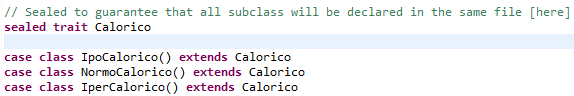
\includegraphics[width=0.5\textwidth]{Immagini/Sealed.png}
	\caption{Sealed}
	\label{fig:sealed}
\end{figure}
